\section{Background}\label{sec:background}

While our approach is architecture neutral, our implementation is based on the Atmel AVR toolchain and focuses on AVR microprocessors. In this section, we survey the stack frame, function call process, and the AVR Toolchain optimization levels.

\subsection{Stack Frame}

The stack consists of stack frames, each corresponding to a function call. A stack frame is created when a function is called, and freed when the function returns. For example, as shown in Figure \ref{fig:stack_frame}, when the \textit{main} function calls the \textit{foo} function, a stack frame will be created for \textit{foo}. First, the return address of \textit{main} will be pushed to the stack, followed by the conflict registers. Next, the local variables and parameters will be pushed to the stack in reverse order of declaration. The stack frame spans the return address through the first parameter. The stack frame pointer, Y, now points to the next available address in the stack. When \textit{foo} finishes execution, the stack frame will be freed, and the stack frame pointer will point back to the position where the return address of the previous stack frame was stored.

\begin{figure}
\centering
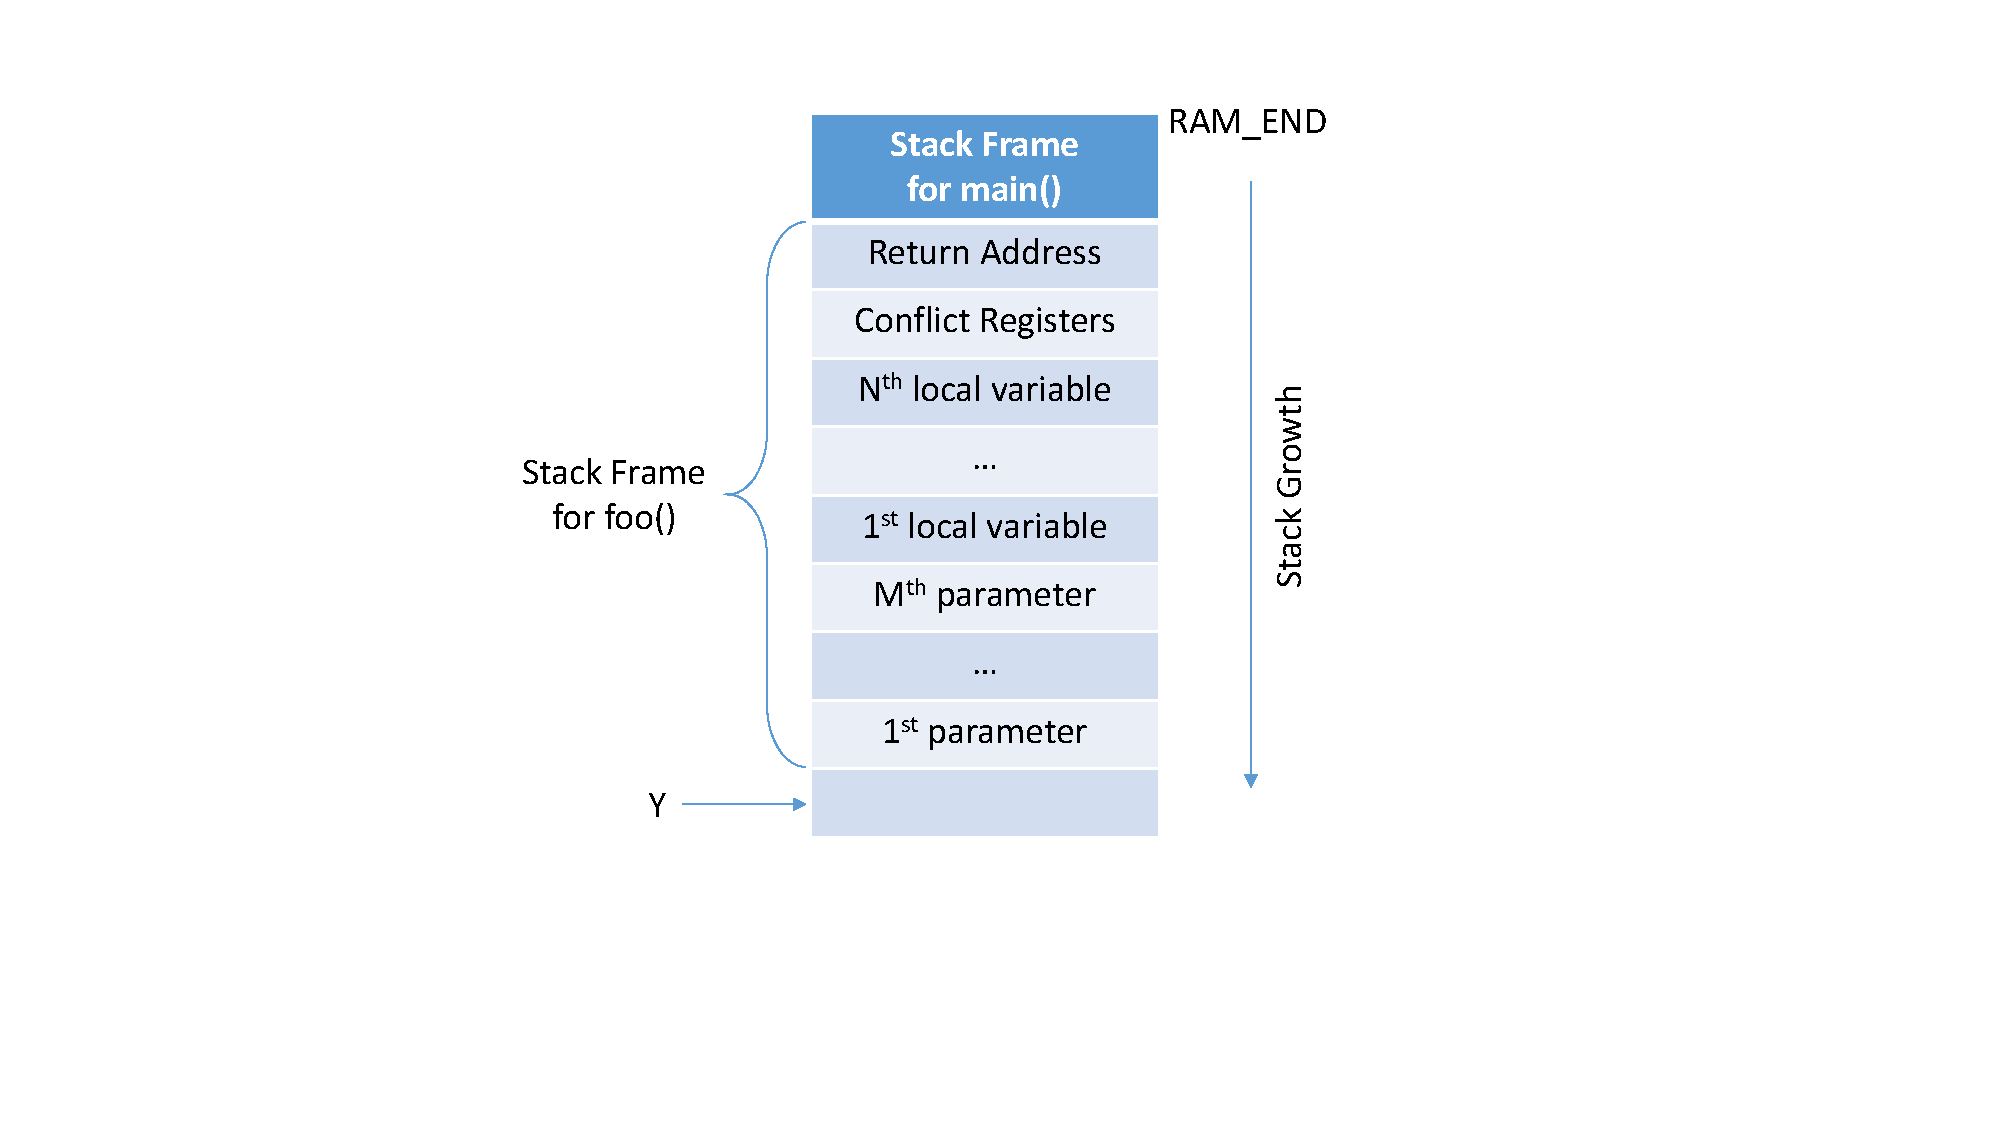
\includegraphics[scale=0.55]{figures/stack_frame_v2.pdf}
\vspace{5pt}
\caption{AVR Stack Frame}
\label{fig:stack_frame}
\end{figure}

\subsection{Function Calls}

All function calls follow the same process and use the system stack to perform most operations, as illustrated in Figure \ref{fig:original_function_operation}. Figure \ref{fig:original_function_operation_process} explains the execution process when a function is called, and Figure \ref{fig:original_function_operation_stack} shows the associated stack changes after each operation is performed. Each rectangle represents two bytes in the stack. The numbers below each stack denote the operation(s) that changed the stack. \texttt{SP} denotes the stack pointer, and \texttt{Y} denotes the stack frame pointer. When a function is called, the return address is automatically pushed onto the stack by one of the function call instructions, \texttt{call}, \texttt{rcall}, or \texttt{icall} (step 1). After the stack frame pointer is pushed (step 2), the stack frame of the function is created by changing the stack pointer and stack frame pointer (step 3). The arguments and local variables are then pushed onto the stack (step 4), and the function begins executing (step 5). The arguments and local variables are released after the function finishes its execution (step 6), and the stack frame pointer is restored (step 7). Finally, the function returns (step 8). The return address is popped and used when one of the function return instructions, \texttt{ret} or \texttt{reti}, is called.

\begin{figure}[h]
        \centering
        \begin{subfigure}[b]{0.4\columnwidth}
                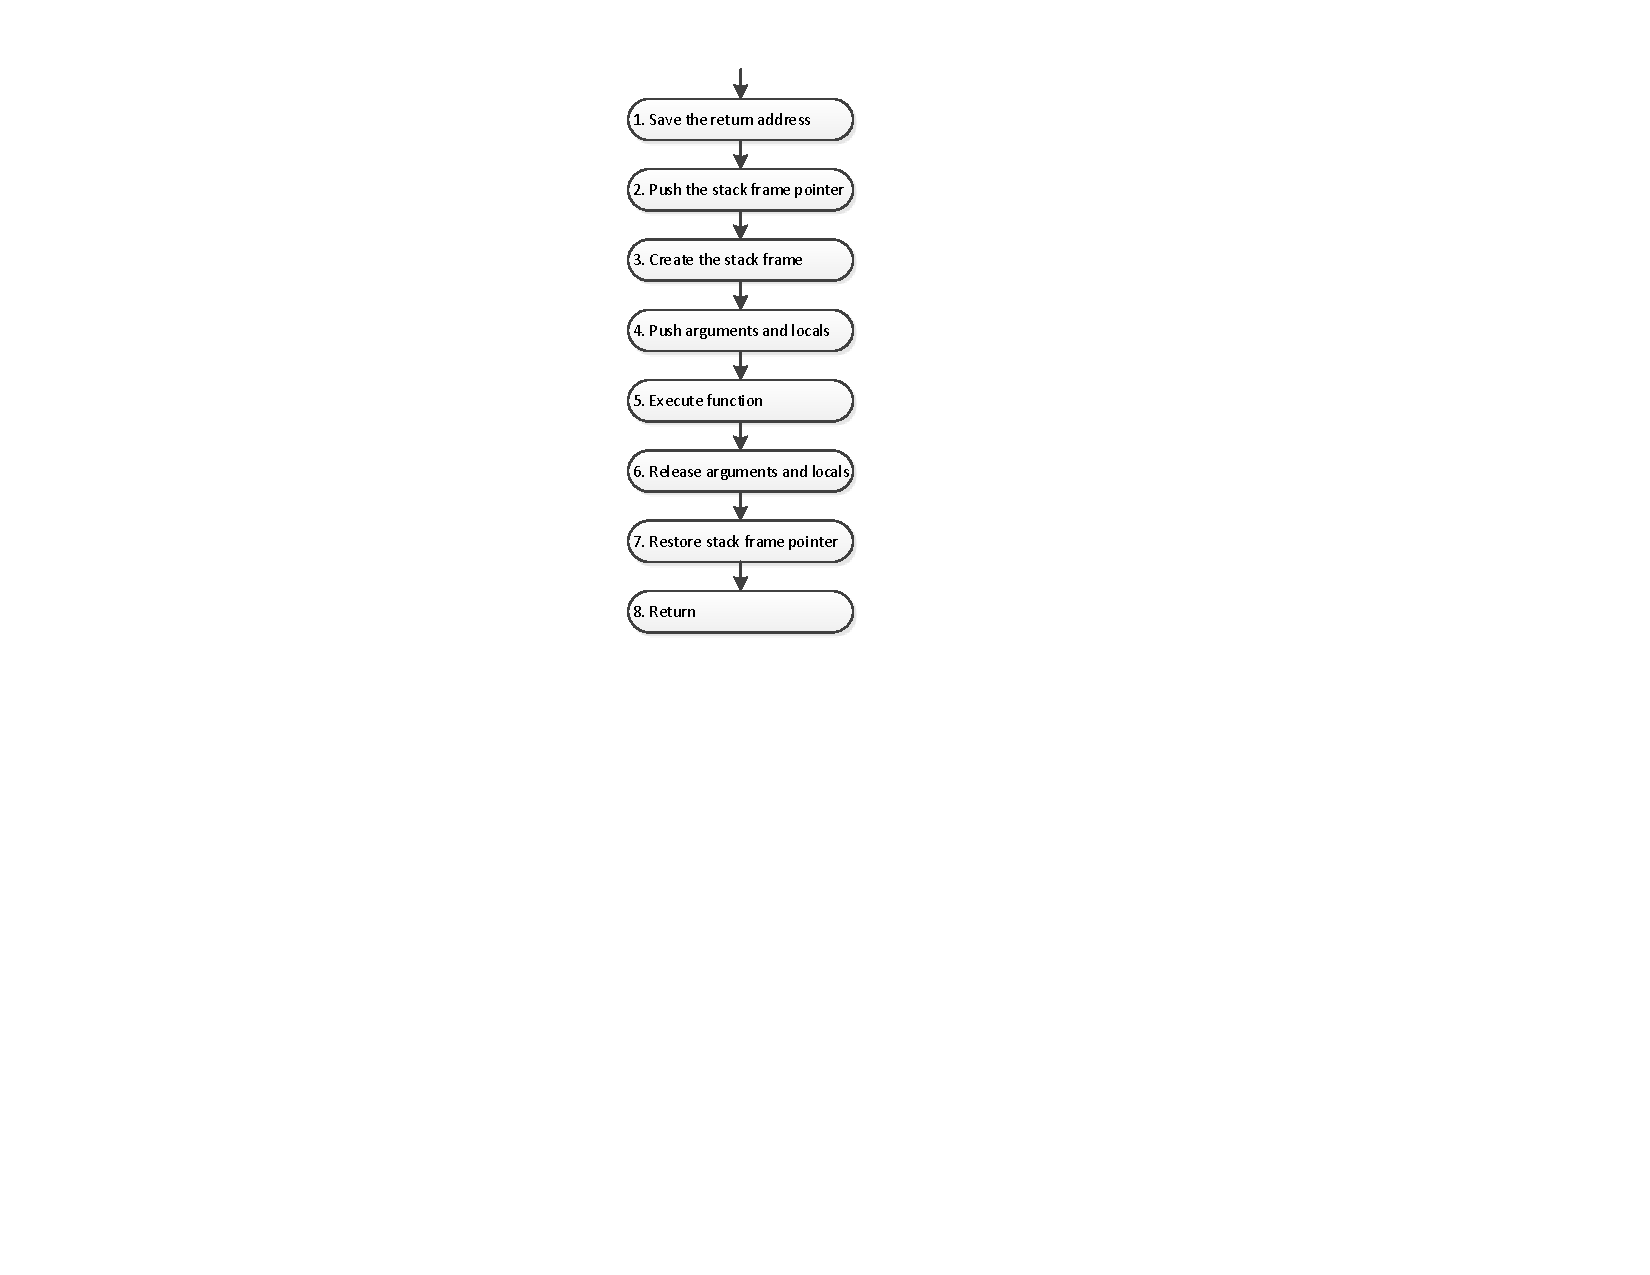
\includegraphics[width=\textwidth, height=12cm]{figures/original_function_operations_process_v3}
                \caption{Process}
                \label{fig:original_function_operation_process}
        \end{subfigure}~
        \begin{subfigure}[b]{0.6\columnwidth}
                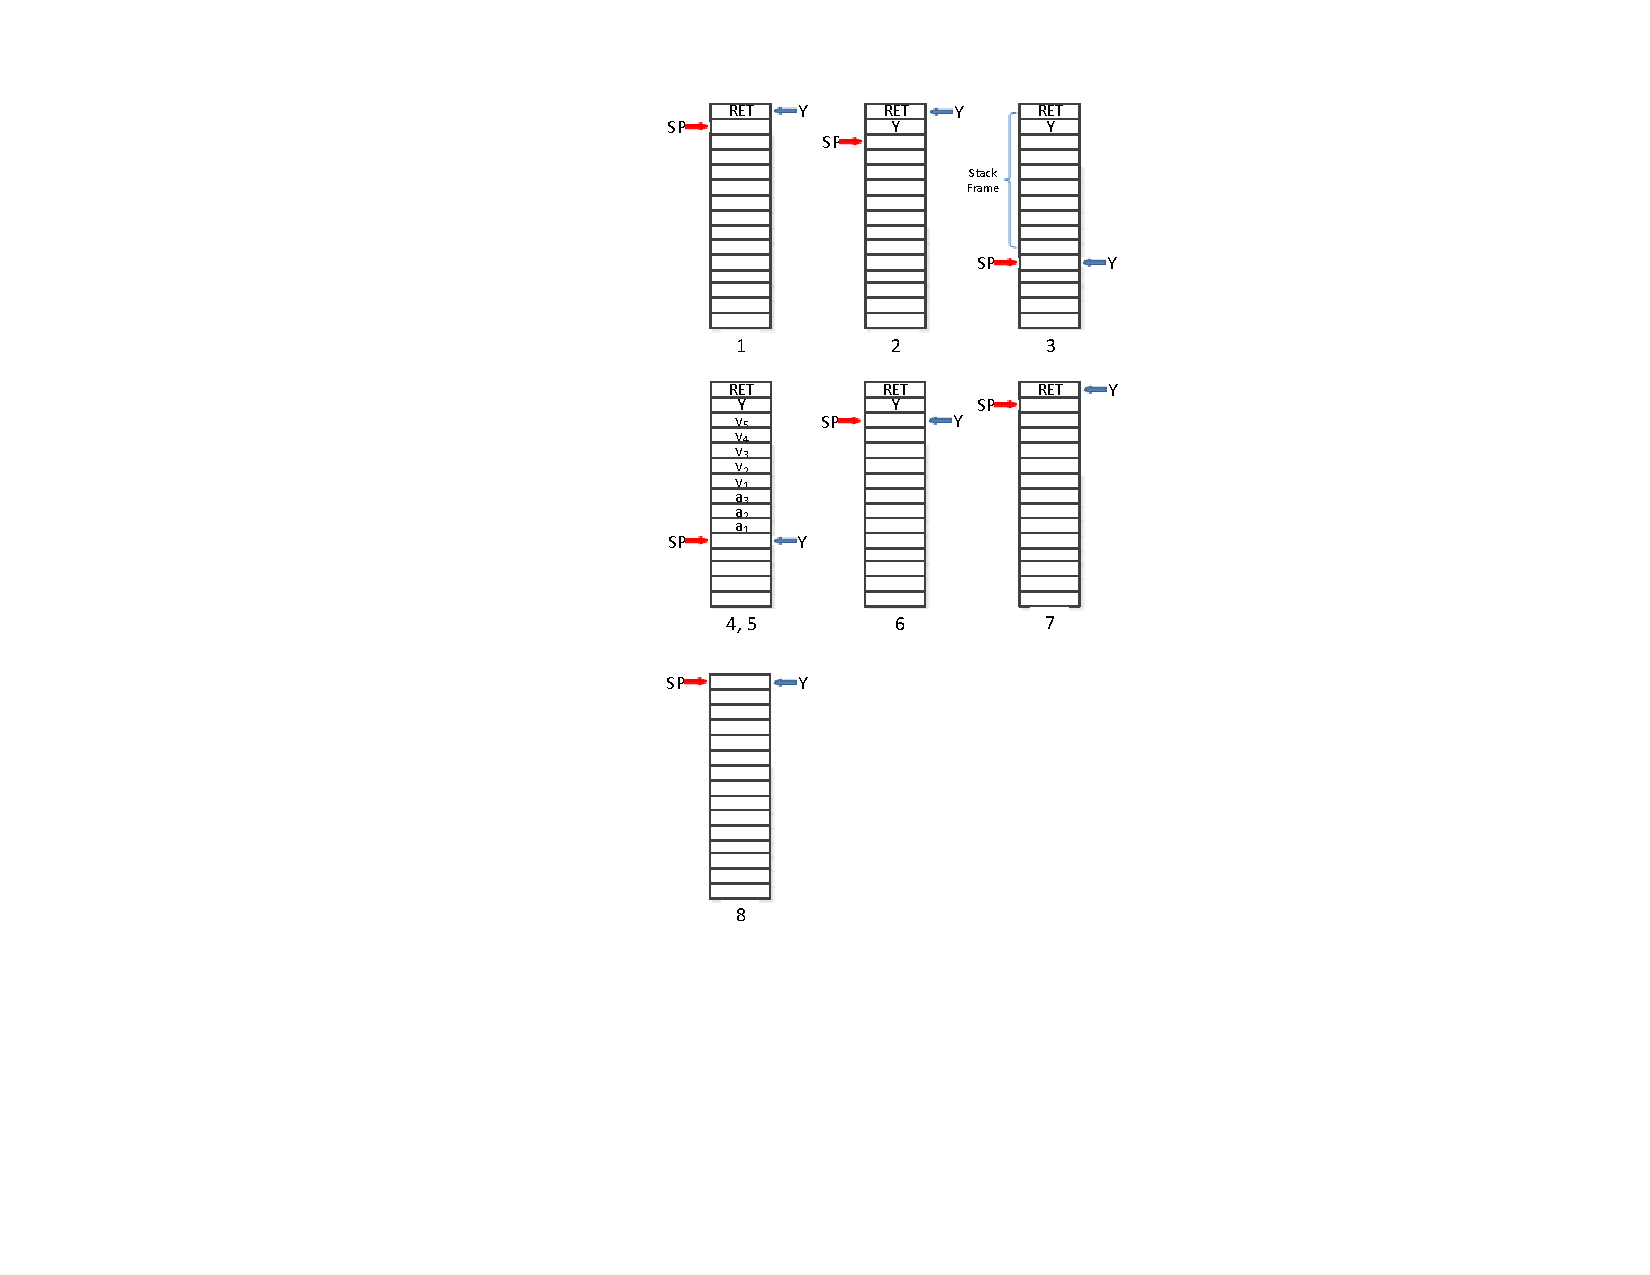
\includegraphics[width=\textwidth, height=11.5cm]{figures/original_function_operations_stack_v2}
                \caption{Stack}
                \label{fig:original_function_operation_stack}
        \end{subfigure}
		\vspace{5pt}
        \caption{Function Execution}\label{fig:original_function_operation}
\end{figure}

\subsection{AVR Toolchain Optimization Levels}

The AVR GCC toolchain is used in our approach. It provides 5 optimization levels, each providing different optimization options. The exception is -O0, which offers no optimization\cite{hoste2008cole}. Our approach is based on modifying unoptimized assembly code generated with the -O0 option. This option makes it more convenient for developing, debugging, and evaluating our approach. However, we plan to extend our approach to other optimization levels in future work.


\begin{comment}
\subsection{AVR Architecture}

AVR microprocessors are based on a modified Harvard architecture~\cite{argade1996apparatus}, which stores instructions and data in physically separate memories, flash memory and SRAM, respectively. Instructions and data are accessed concurrently through separate memory buses. Flash memory is non-volatile and offers high capacity, but slow access speed, and is used to store executable programs composed of AVR instructions. The SRAM is volatile and offers low capacity, but fast access speed, and is used to store data used by the executable programs at runtime. The ATmega644 includes 64KB of flash memory, 4KB of SRAM, a 16-bit instruction bus, and an 8-bit data bus.

\subsubsection{AVR SRAM}

The on-board SRAM of the ATmega644 has an address range of 0x0100 to 0x10FF, as shown in Figure \ref{fig:ram_map}. The SRAM is partitioned into sections, each used to store different types of data. The \textit{.data} section is used to store initialized static variables and global variables. The \textit{.bss} section is used to store uninitialized static and global variables. The pre-allocated SRAM usage is the sum of the sizes of the .data and .bss sections. The remaining space in SRAM is shared by the heap and stack sections. The \textit{heap} section is used to store dynamically allocated memory, e.g. when \textit{malloc()} is called~\cite{goldt1995linux}. The heap grows ``upward'', towards the higher address range. The \textit{stack} section is used to store a return address, actual parameters, conflict registers, local variables, and other information. The stack grows ``downward'', from \textit{RAM\_END}, address 0x10FF, towards the lower address range.
\begin{figure}
\centering
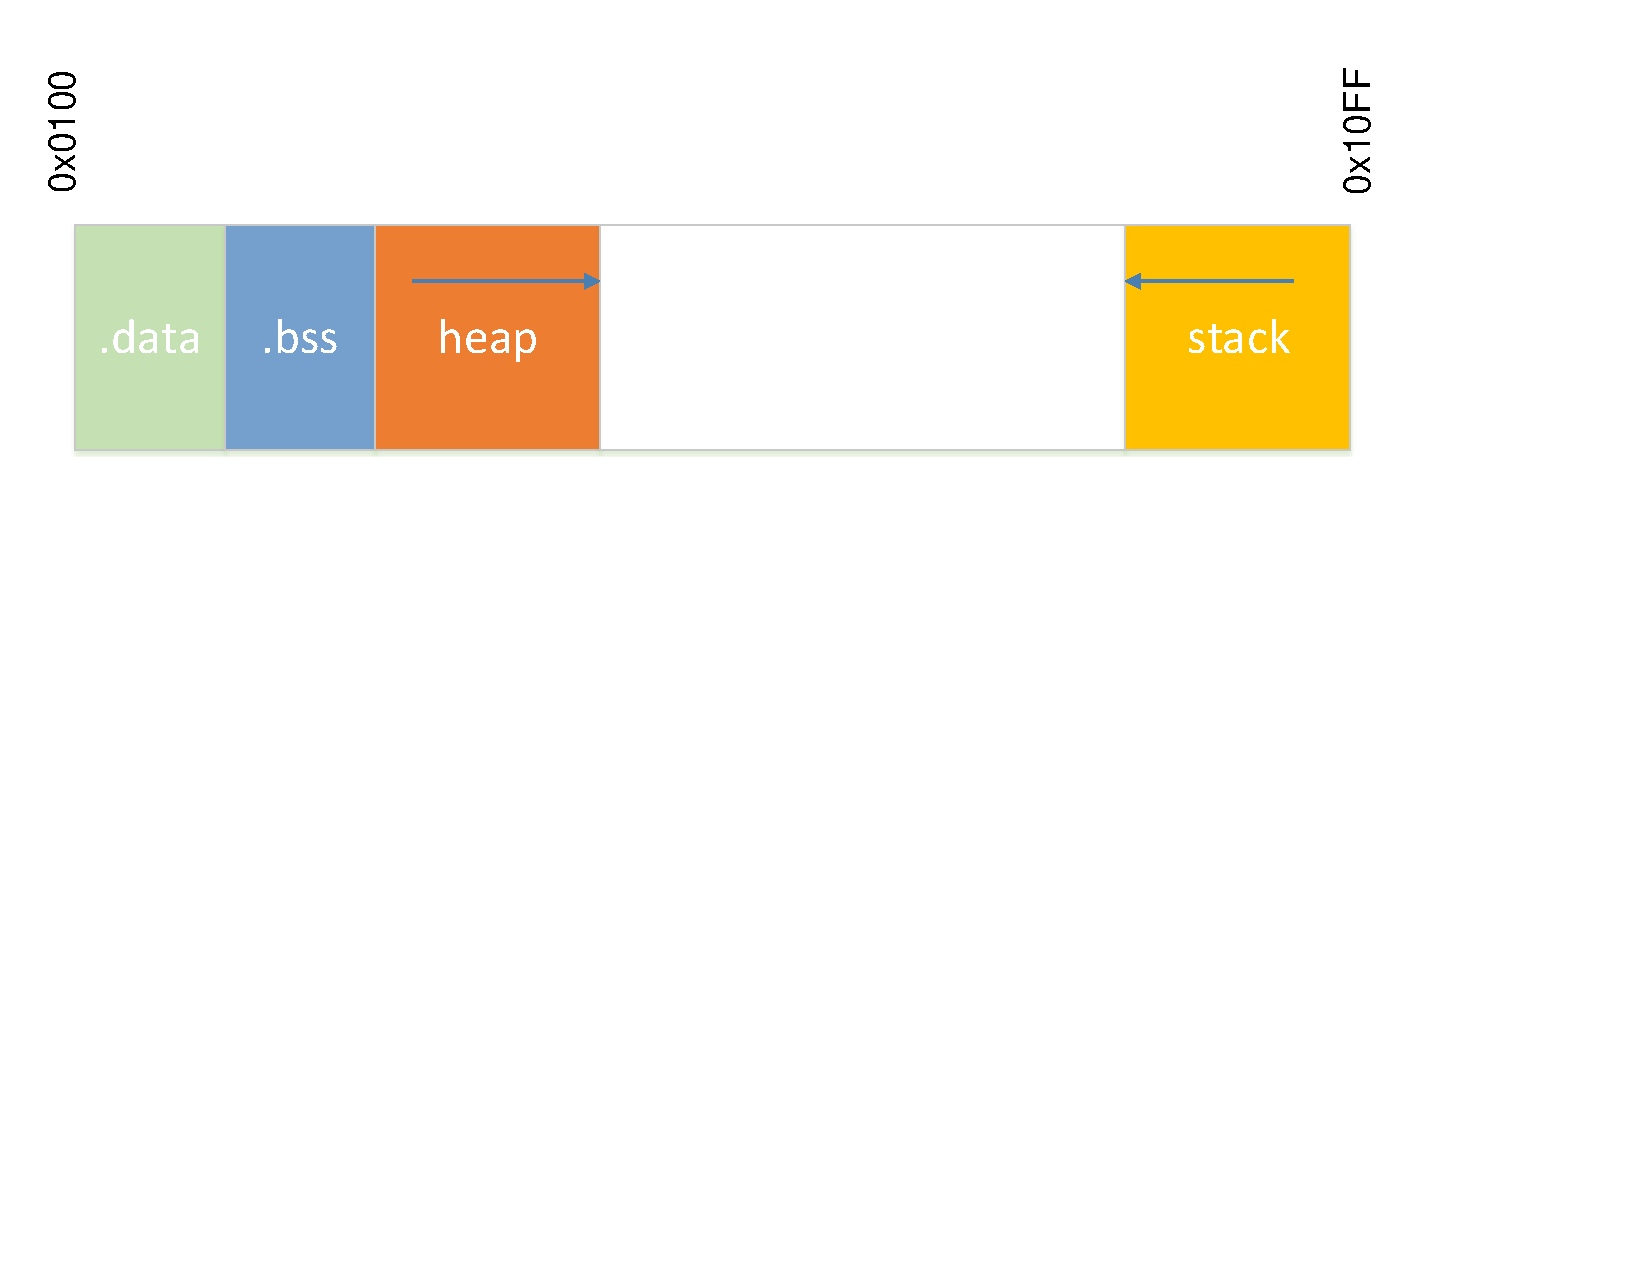
\includegraphics[width=0.5\textwidth]{figures/Memory_model.pdf}
\caption{AVR RAM Map}
\label{fig:ram_map}
\end{figure}

\subsubsection{Stack Frame}

The stack consists of stack frames, each corresponding to a function call. Each stack frame is created when a function is called, and freed when the function returns. For example, as shown in Figure \ref{fig:stack_frame}, when the \textit{main} function calls the \textit{foo} function, a stack frame will be created for \textit{foo}. First, the return address of \textit{main} will be pushed to the stack, followed by the conflict registers. Next, the local variables and parameters will be pushed to the stack in reverse order of their declarations. The stack frame spans the return address through the first parameter. The stack frame pointer, Y, now points to the next available address in the stack. When \textit{foo} finishes execution, the stack frame will be freed, and the stack frame pointer will point back to the position where the return address of the previous stack frame was stored.

\begin{figure}
\centering
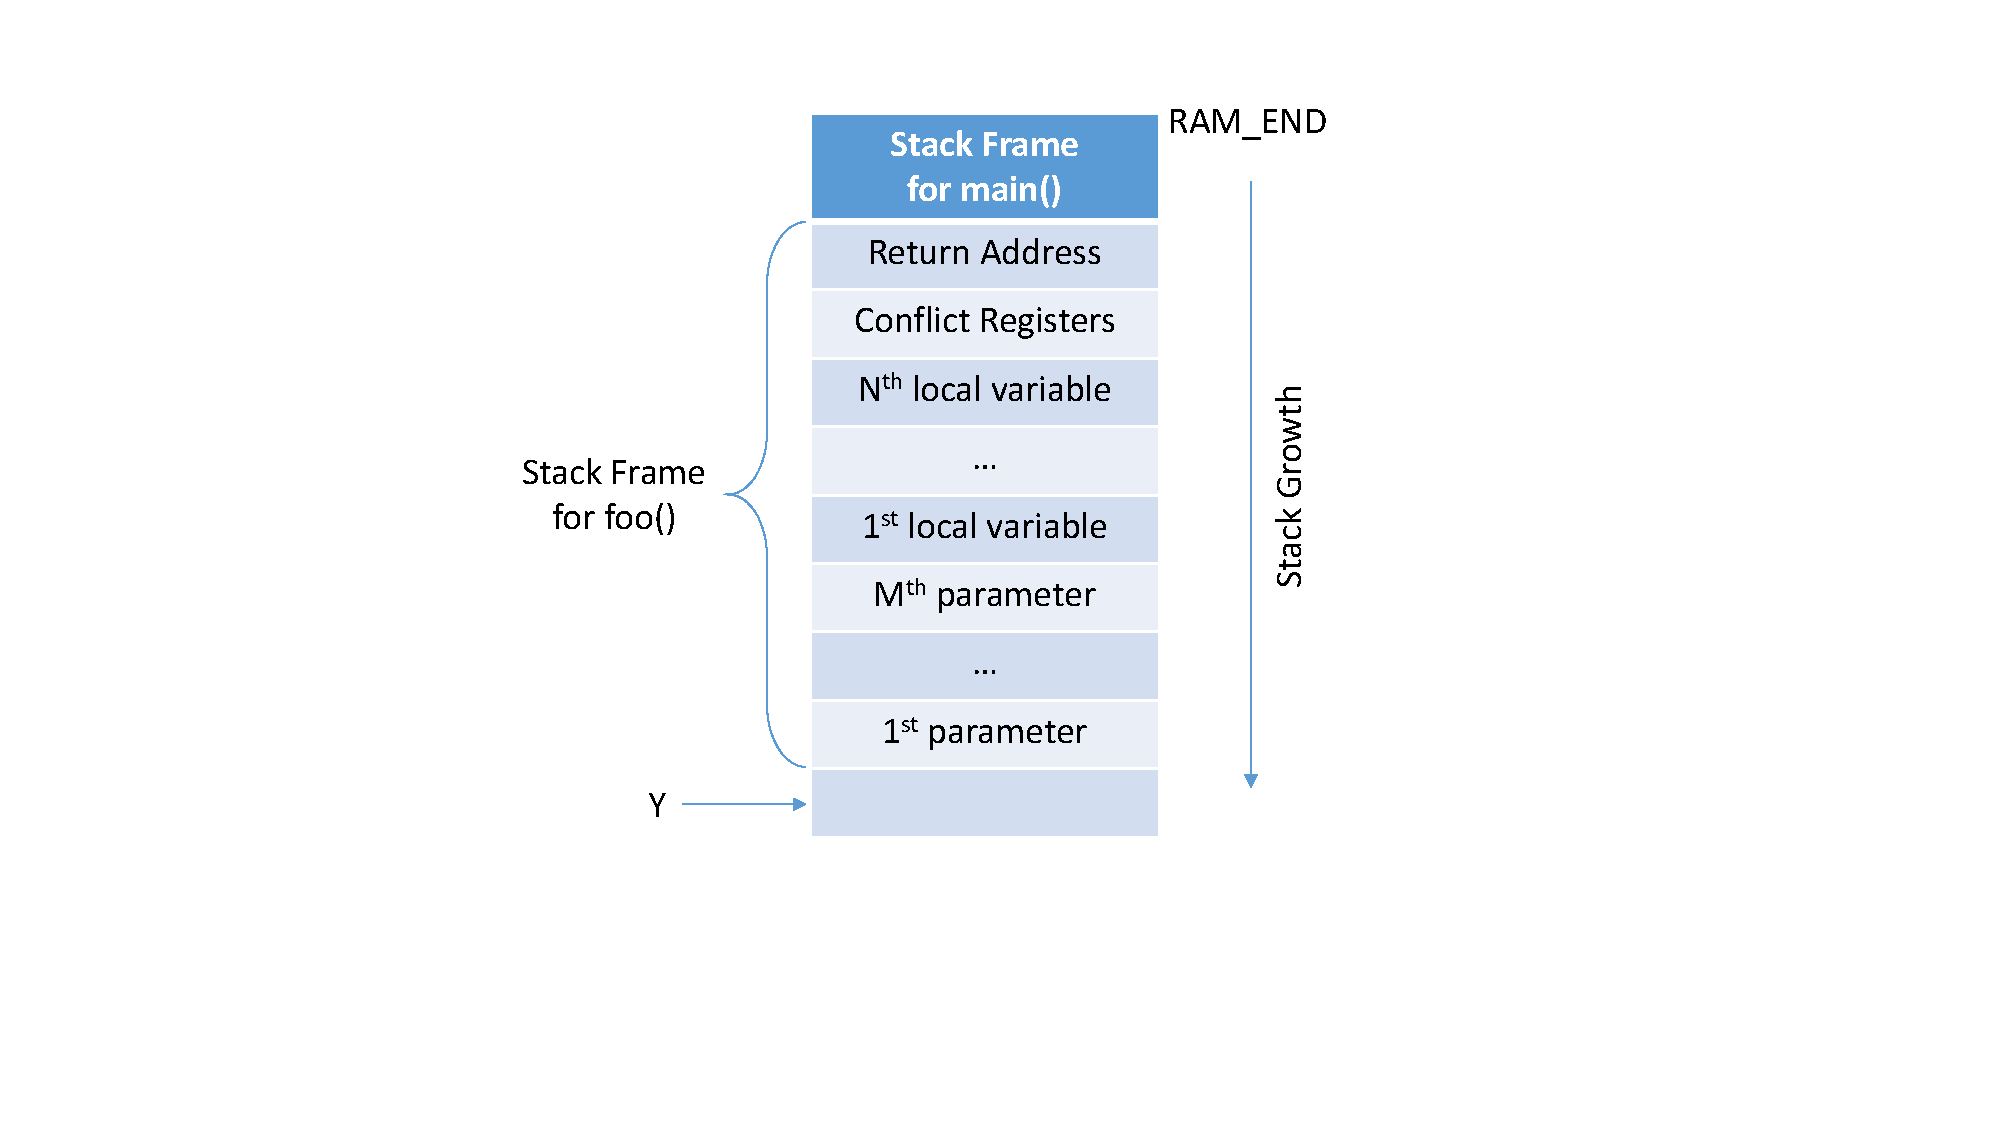
\includegraphics[scale=0.55]{figures/stack_frame_v2.pdf}
\caption{AVR Stack Frame}
\label{fig:stack_frame}
\end{figure}

\subsubsection{Registers}

AVR microprocessors have two types of registers, general-purpose registers and I/O registers. 

General-purpose registers are used for arithmetic operations, such as adding, subtracting, and comparing numbers, as well as indexing and setting long jump destinations. The ATmega644 has 32 general-purpose registers, R1 through R32, which are mapped into the first 32 locations of the RAM space, and can be directly used in assembly commands. Some general-purpose registers are used for special purposes; for example, R29 and R28 store a 16-bit address, the Y pointer, to indicate the top of the current stack frame. (The use of the Y pointer will be explained in the next subsection). The use of these registers is compiler-dependent. For example, AVR-GCC uses R24 and R25 to store the return value of each function call. We attempt to limit the number of registers manipulated by our approach to reduce the cost of saving and restoring the conflict registers.

The I/O registers are used to control the internal peripherals of the AVR microprocessor.
The ATmega644 has 64 I/O registers, mapped into the next 64 locations of the SRAM space, \textit{0x20} through \textit{0x5F}. Again, some I/O registers are used for special purposes; for example, AVR-GCC uses \textit{0x3E} and \textit{0x3D} as the stack pointer (SP), which indicates the current top of the stack.

\subsection{Function Calls}

All function calls follow the same process and use the system stack to perform most operations, as illustrated in Figure \ref{fig:original_function_operation}. Figure \ref{fig:original_function_operation_process} explains the execution process when a function is called, and Figure \ref{fig:original_function_operation_stack} shows the associated stack changes after each operation is performed. Each rectangle represents two bytes in the stack. The numbers below each stack denote the operation(s) that changed the stack. \texttt{SP} denotes the stack pointer, and \texttt{Y} denotes the stack frame pointer. When a function is called, the return address is automatically pushed onto the stack by one of the function call instructions, \texttt{call}, \texttt{rcall}, or \texttt{icall} (step 1). After the stack frame pointer is pushed (step 2), the stack frame of the function is created by changing the stack pointer and stack frame pointer (step 3). The arguments and local variables are then pushed onto the stack (step 4), and the function begins executing (step 5). The arguments and local variables are released after the function finishes its execution (step 6), and the stack frame pointer is restored (step 7). Finally, the function returns (step 8). The return address is popped and used when one of the function return instructions, \texttt{ret} or \texttt{reti}, is called.

\begin{figure}[h]
        \centering
        \begin{subfigure}[b]{0.4\columnwidth}
                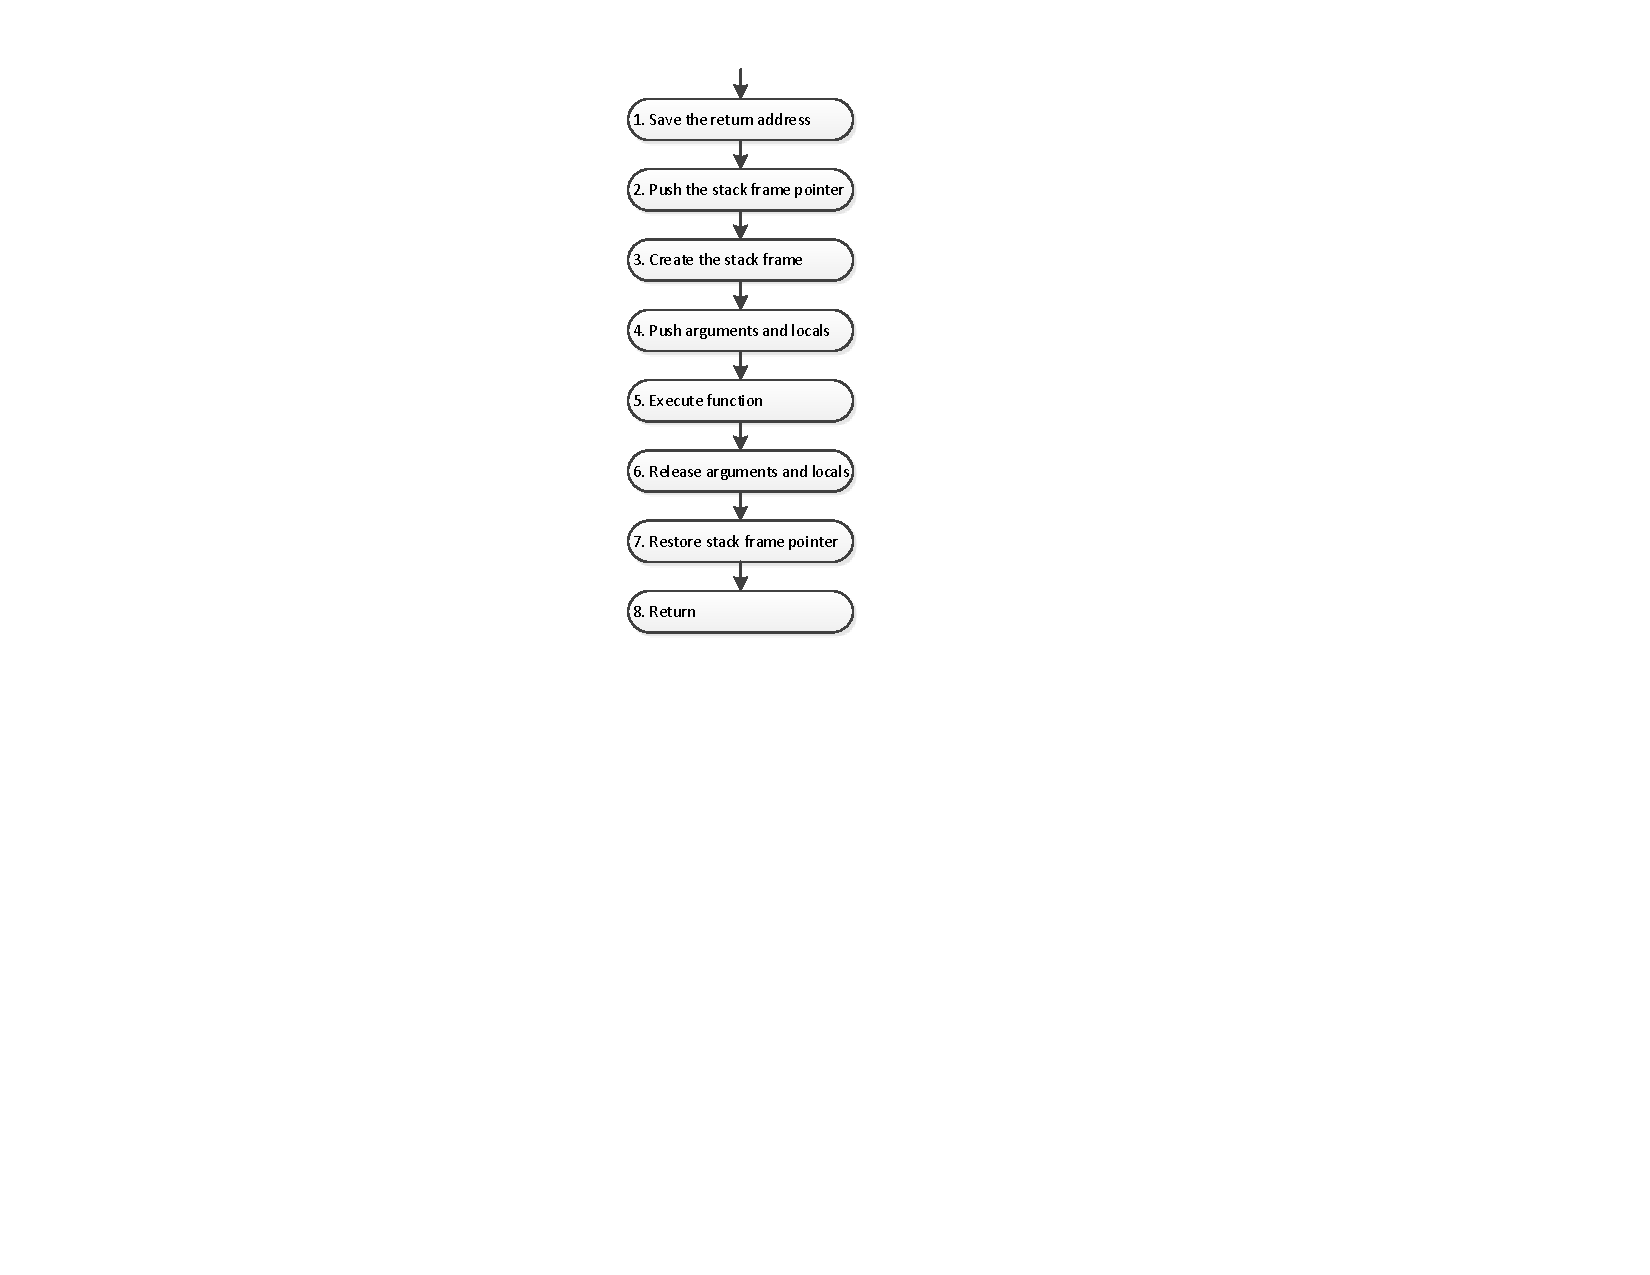
\includegraphics[width=\textwidth, height=12cm]{figures/original_function_operations_process_v3}
                \caption{Process}
                \label{fig:original_function_operation_process}
        \end{subfigure}~
        \begin{subfigure}[b]{0.6\columnwidth}
                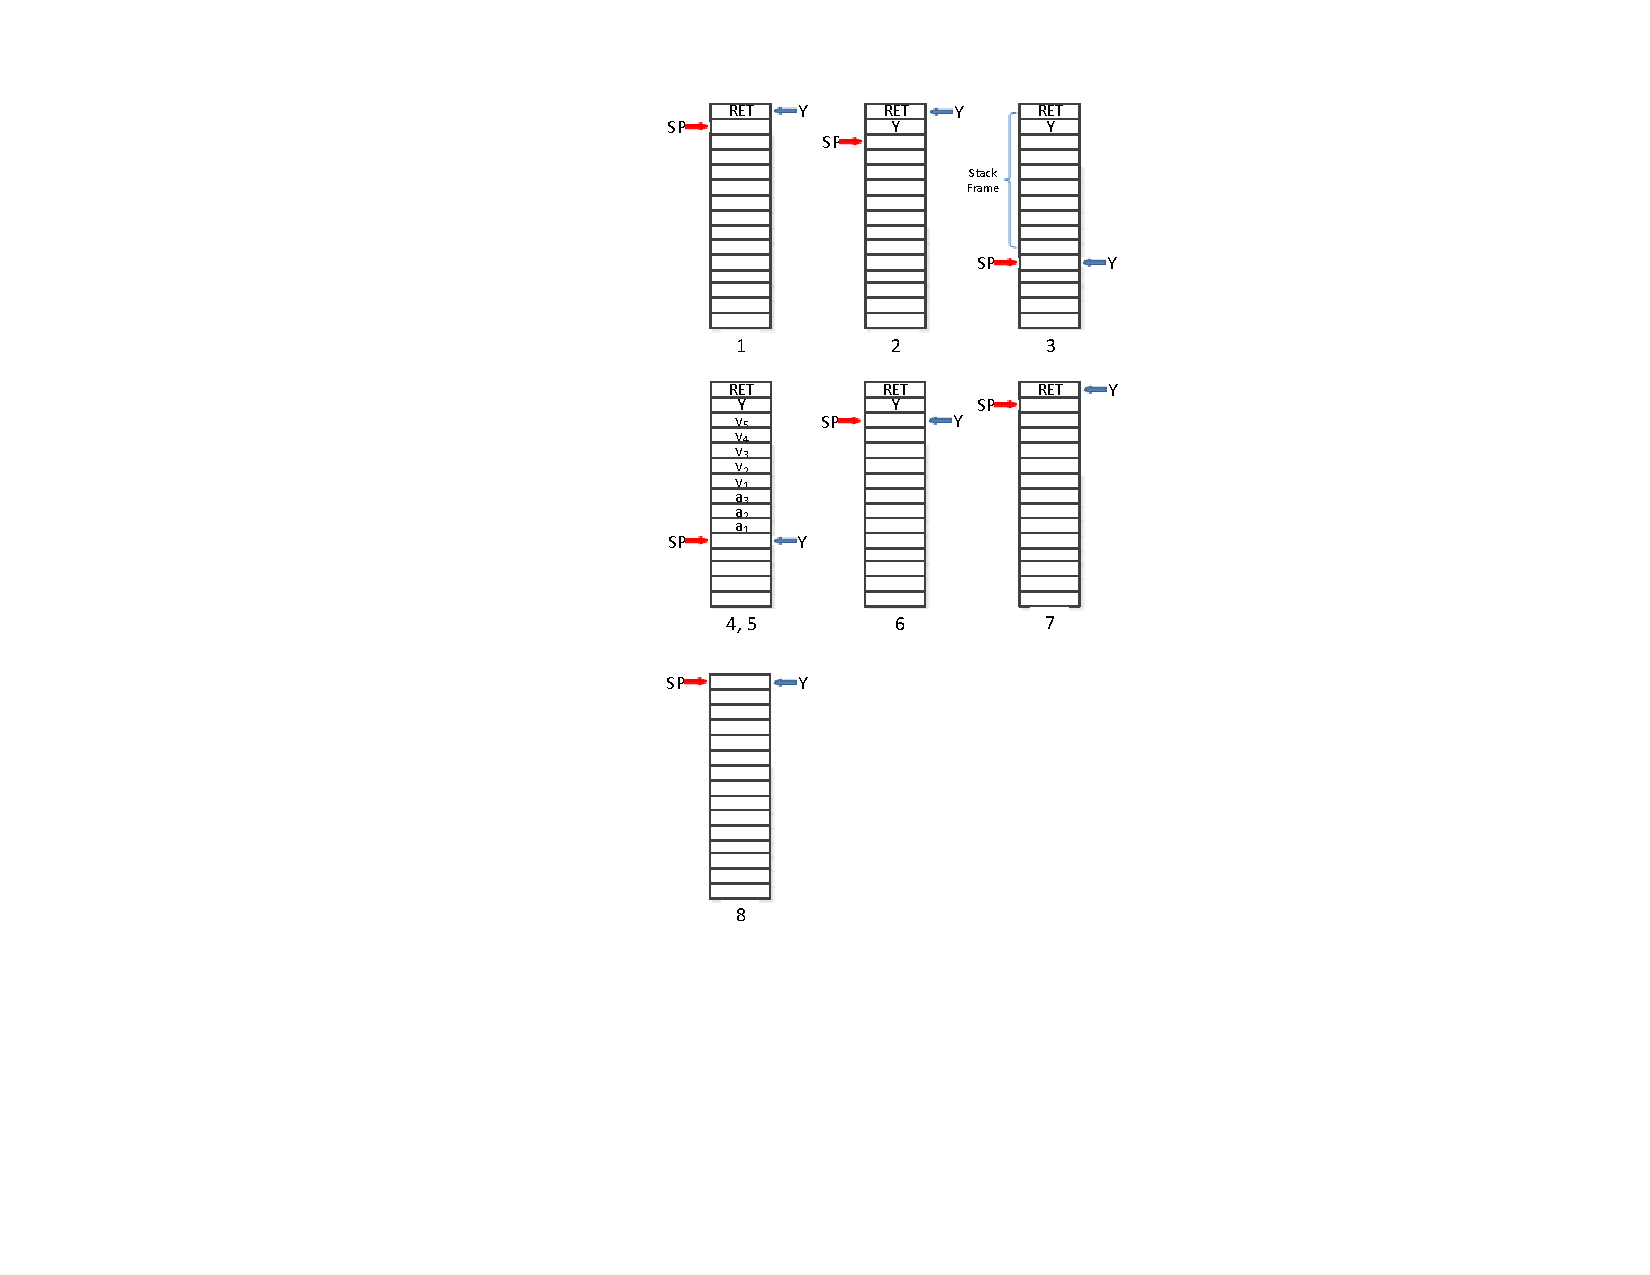
\includegraphics[width=\textwidth, height=11.5cm]{figures/original_function_operations_stack_v2}
                \caption{Stack}
                \label{fig:original_function_operation_stack}
        \end{subfigure}
        \caption{Function Execution}\label{fig:original_function_operation}
\end{figure}

\subsection{Atmel AVR Toolchain}

The Atmel AVR toolchain is a collection of tools used to generate executable programs for AVR microprocessors. The toolchain consists of the following tools.

\begin{itemize}

\item \textit{avr-gcc}, an extension of GNU GCC, is a cross compiler, which translates high-level C or C++ code to assembly code for AVR microprocessors.

\item \textit{avr-as} is an assembler, which translates AVR assembly code to an object file.

\item \textit{avr-ld} is a linker, which uses a linker script to combine object modules into an executable image suitable for loading into the flash memory of an AVR microprocessor. By using a customized linker script, the default locations and sizes in SRAM can be changed. New memory sections may also be added~\cite{sram}.

\item \textit{avr-libc} is a standard C library, which contains standard C routines, as well as additional AVR-specific library functions.

\end{itemize}

As a matter of convenience, the AVR toolchain can be used to compile, assemble, and link C programs in a single command. However, in order to modify the assembly code of an AVR application and use a customized linker script, these steps are performed individually.


AVR GCC provides 5 optimization levels, -O0, -O1, -O2, -O3, and -Os, each providing different optimization options. The exception is -O0, which offers no optimization\cite{hoste2008cole}. Our approach is based on modifying unoptimized assembly code generated with the -O0 option. This option makes it more convenient for developing, debugging, and evaluating our approach. However, we plan to extend our approach to other optimization levels in future work.

\end{comment}